\chapter{Metropolis Method}\label{ch:metropolis}

The fundamental laws of classical physics suggest that the future is uniquely determined by the present state and there is no room for stochastic variables. If the degree of freedom is small enough, we can predict the future of the system at least it is not a distance future. The necessity of stochastic variables in classical physics is due to our ignorance.  When the system consists of many particles, as many as $10^{23}$, interacting among themselves, it is practically impossible to predict future of the system precisely.  Fortunately, many physical quantities we are interested in do not depend on the detailed state of individual particles.  Think of the air around us.  We are mostly interested in its temperature and pressure.  Nobody asks what is the position and velocity of individual oxygen molecules.
Nevertheless the temperature and pressure (macroscopic states) are determined by the state of the molecules in the air (microscopic states). The rigorous relations between microscopic states and macroscopic states are very complicated.  Statistical mechanics was devised to make some intuitive connection between microscopic states and macroscopic states.\cite{sm1,sm2}  The state of a microscopic system is described by stochastic variables. For example, the velocity of the molecules in the air is a stochastic variable for which a probability distribution is constructed based on the fundamental laws of  physics at the microscopic scale. Once we find the probability distribution, we calculate the mean value which is regarded as a macroscopic quantity.  In other words, we don't solve the Newton's  equations of motion to find the position and velocity of all particles.  Instead we treat the position and velocity as stochastic variables and we somehow find the corresponding probability distribution consistent to the Newtons' laws of motion.

Mathematical approach to stochastic system requires a bit of additional tasks since we need to find probability distributions and various statistical quantities such as mean and variance using the probability distribution. On the other hand, computational approach is rather straight forward.  We just generate a large set of random numbers corresponding to microscopic states and construct the probability distribution.  The calculation of mean and variance is essentially addition of many random numbers.  Computers are very good at repeating simple operations many times and do it very quickly.  We call such approach \textit{Monte Carlo simulation}\cite{monte_carlo_methods}  after the famous casino city in Monaco.\cite{monte_carlo_methods}  In this chapter, a few simple examples are introduced.

The present interpretation of quantum mechanics inherently involves stochastic variables. We can investigate quantum systems using random numbers (quantum Monte Carlo simulation).  We will discuss it in a later chapter.


\section{Metropolis Algorithm for Thermal Equilibrium}

When a system is in a thermal equilibrium at temperature $T$, all macroscopic quantities remain constant in time and all macroscopic flow such as heat flow and particle current vanish.  It looks no activity in the system.  However, if we look at the system at a microscopic level, the atoms are moving and the microscopic state of the system is evolving in time rather rapidly.  Macroscopic measurement devices simply do not have a sufficient resolution  to see such rapidly changing quantities. Instead the devices measure the time-averaged quantities.  For classical systems, a physical quantity is in general a function of a set of coordinates $\{q_i(t)\}$ and momenta $\{p_i(t)\}$ and the time-average of a physical quantity $A$ is defined by
\begin{equation}
\mean{A} = \frac{1}{t} \int_0^t A[q_1(\tau),q_2(\tau), \cdots,  p_1(\tau), p_2(\tau), \cdots] \md \tau
\end{equation}
The time average is done rather quickly in our scale, say a micro second.  However, it is almost infinitely long in the microscopic world.  Atoms in solid oscillate $10^{13}$ times in 1 second.   It is difficult to simulate the motion of atoms long enough to get macroscopic time average even with modern supercomputers.

Statistical mechanics offers us an alternative method to calculate the macroscopic average.  The probability that the system is found to be in a microscopic state $\psi_i$ whose energy is $E_i$ is given by the Boltzmann distribution
\begin{equation}\label{eq:Boltzmann}
P_i = \frac{1}{Z} \me^{-\beta E_i}
\end{equation}
where $\beta=1/\kB T$.  The normalization constant $Z=\sum \me^{-\beta E_i}$ is called the partition function.  Then, the mean can be computed by
\begin{equation}
\mean{A} = \sum_i A_i P_i = \frac{1}{Z}\sum_i A_i \me^{-\beta E_i}.
\end{equation}
This summation is done over  all microscopic states.  Unfortunately, the number of microscopic states is huge and the exact enumeration is impossible.  However, a reasonably large but finite random sampling is good enough to get accurate mean value.  If we want evaluate
the mean of stochastic variable $\hat{A}$, we pick $N$ random numbers $A_i$
\begin{equation}
\mean{A} \approx \frac{1}{N} \sum_{j \in \mathcal{S}} A_j
\end{equation}
where $\mathcal{S}$ is a subset of the all possible microscopic states chosen at random according to the probability (\ref{eq:Boltzmann}) and $N$ is the number of samples in $\mathcal{S}$.  A question is how to find the subset $\mathcal{S}$.
Metropolis \textit{et al.}\cite{metropolis1953} found a good way.

We want to take a finite number of samples from the all possible microscopic states in a way that the samples are consistent with thermodynamic equilibrium.  The chance that a particular state $\psi_i$ is sampled must be proportional to the Boltzmann factor $\me^{-\beta E_i}$.
Making a question more concrete, suppose that we pick a state $\psi_i$ at random.  Then, which state should we pick next.  If you just pick at random, you don't satisfy the equilibrium distribution.  In Chapter 14, we learned how to pick a random number from a desired distribution.  Unfortunately, we cannot use it here since the distribution is given as a function of energy instead of $A_i$.  We can pick an energy in accordance with the Boltzmann distribution.  However, we can not construct the corresponding microscopic state from the energy since many states have the same energy.

When the system is at an thermal equilibrium, any transition must satisfy the detailed balance\cite{detailed_balance}
\begin{equation}
p_{i \rightarrow j} \me^{-\beta E_i} = p_{j \rightarrow i} \me^{-\beta E_j} \qquad \Rightarrow \qquad \frac{p_{i \rightarrow j}}{p_{j \rightarrow i}}= \me^{-\beta (E_j-E_i)}
\end{equation}
where $p_{i \rightarrow j}$ is the transition probability from state $i$ to $j$.  The absolute value of the transition probability is not necessary to satisfy the detailed balance.  We need to know only the relative transition probability.  So, we use a simple one
\begin{equation}
p_{j \rightarrow i} = 1, \qquad p_{i \rightarrow j}=\me^{-\beta (E_j-E_i)}
\end{equation}
for $E_j>E_i$.  For the other case $E_i<E_j$.  We simply swap $i$ and $j$.   Based on this idea, the following algorithm sample the microscopic states satisfying the detailed balance and thus the Boltzmann distribution.

\bigskip
\begin{myalgobox}
\Algorithm{Metropolis Algorithm}\label{algo:metropolis}

\medskip
\begin{minipage}{5.5in}
\small
\begin{enumerate}
\item Pick an initial state $\psi_1$ at random.  Starting $i=1$, repeat the following procedure.
\item Pick a candidate state $\psi_\text{c} $ at random. We consider the jump from $\psi_i$ to $\psi_\text{c}$.
\item Evaluate energy difference $\Delta E=E_{c}-E_{i}$.
\item If $\Delta E \le 0$, then the transition is accepted. Let $\psi_{i+1}=\psi_{c}$.  Increment $i$ and go to step 2.
\item If $\Delta E > 0$, generate a uniform random number $r$  between 0 and 1.
\item If $\me^{-\beta \Delta E} > r$, then the transition is accepted.  Let $\psi_{i+1}=\psi_{c}$.  Increment $i$ and go to step 2.
\item Otherwise, the transition is rejected.  Discard the candidate state and start over from Step 2.
\end{enumerate}
After $N$ iterations, we have a set of sample $\{\psi_1, \cdots, \psi_N\}$ which is consistent with the Boltzmann distribution.  This algorithm is known as the Metropolis method.
\end{minipage}
\end{myalgobox}


\bigskip


\bigskip
\begin{example}{Maxwell Velocity Distribution}

\medskip
\noindent
Consider a one-dimensional ideal gas in a thermal equilibrium at temperature $\kb T$.  The velocity of the gas particles (mass=$m$) is distributed in the Maxwell distribution
\begin{equation}
\rho(v)= 
\frac{m}{\sqrt{2\pi \kB T}} \me^{-m v^2/2 \kB T}.
\end{equation}
It can be obtained from the Boltzmann distribution with  $E=\frac{1}{2} m v^2$. We can can sample the velocity 
directly using the normally distributed random number discussed in Chapter 14.  Here, we try to get the Maxwell velocity distribution using the Metropolis method.  In Program \ref{prog:maxwell_metropolis} the velocity is sampled using the Metropolis algorithm.  The jump of the velocity $\Delta v$ is chosen at random between $-0.5$ and $0.5$. 100000 velocities are sampled and compared with the exact Maxwell distribution.  Since the velocity is a continuous variable, the probability distribution is expressed in a histogram.
The result is shown in Fig. \ref{fig:maxwell_metropolis}. The Metropolis method successfully obtained the Maxwell distribution.  The small discrepancy is due to the finite sampling.  A better result can be obtained if a larger number of samples are generated.

\begin{figure}
\centering
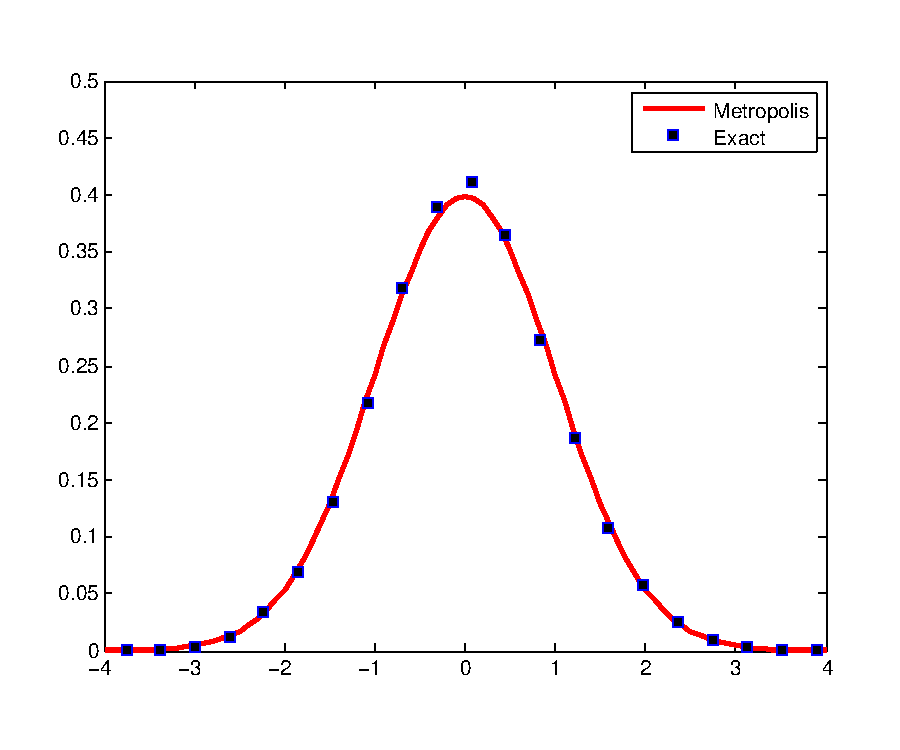
\includegraphics[width=2.5in]{17.Metropolis/maxwell_metropolis.pdf}
\caption{Velocity distribution generated by the Metoropolis method.  The red line plots the Maxwell distribution.}
\label{fig:maxwell_metropolis}
\end{figure}
\end{example}

\noindent
\section{Applications in Physics}

\subsection{Ferromagnetic Phase Transition:  2D Ising Model}



We are familiar with a permanent magnet and we know that it is made of iron or some other transition metals. The permanent magnet has non-zero  magnetization, known as spontaneous magnetization,  even in the absence of external magnetic field. However, the spontaneous magnetization vanishes above a critical temperature (named as he Curie temperature).  This phase transition was explained by a simple model.  It turns out that the model can explain many other phase transitions such as binary alloys and even neural networks.  The model is called the Ising model named after Ernest Ising.

Here we consider the Ising model in two-dimensional square lattices.  The magnetization is caused by the electron spins. In the Ising model, a spin degree of freedom simply takes one of two states denoted by $\sigma=\pm 1$ corresponding to spin ``up'' and ``down''.  The spins interact among themselves but only those at the nearest neighbor sites.  The energy of  the system is defined as
\begin{equation}\label{eq:ising_H}
H = - J \sum_{\langle \lambda, \lambda' \rangle} \sigma_\lambda \sigma_{\lambda'}
\end{equation}
where $\lambda$ denotes a lattice point and $\langle \lambda, \lambda' \rangle$ represents a possible nearest neighbor pair.
$J$ is a coupling constant and positive for ferromagnetic materials.  For example, the four pairs in the left panel of Fig \ref{fig:ising_model1} has energy $-4J$ and another four pairs in the right panel has $0$ energy.  When all spins are in the same direction,
that is $\sigma_\lambda=1, \forall \lambda$ or $\sigma_\lambda=-1, \forall \lambda$, the energy per spin is $-2J$, which is the lowest.
Hence, when $T=0$, the spins are all aligned.

A microscopic state is uniquely specified by a spin configuration $S_i=\{ \sigma_1, \sigma_2, \cdots, \sigma_L \}, i=1, \cdots, 2^L$ where $L$ is the number of spins in the system.  For example, $S_1=\{1,1,1,1, \cdots, 1\}$, $S_2=\{-1, 1, 1, \cdots, 1\}$ and so on.   For each configuration, the corresponding energy of the state is denoted as $E_i$.  The magnetic moment for the configuration $S_i$ is given by
\begin{equation}
M_i = \sum_\lambda \sigma_\lambda.
\end{equation}

The macroscopic quantities are the thermal average of the corresponding microscopic values. The energy of the system is
\begin{equation}\label{eq:ising_E}
\mean{E} = \sum_i E_i\, \me^{-\beta E_i}/Z
\end{equation}
and the magnetization 
\begin{equation}\label{eq:ising_M}
\mean{M} = \sum_i M_i\, \me^{-\beta E_i}/Z.
\end{equation}
Another interesting quantity is heat capacity
\begin{equation}\label{eq:ising_C}
\mean{C} = \kB \beta^2 (\mean{E^2}-\mean{E}^2).
\end{equation}
We are interested in how these quantities vary as temperature changes.

Analytic theory was difficult except for one-dimensional Ising system.  Onsagar was able to solve the two-dimensional system.  The system shows spontaneous magnetization below a critical temperature $\displaystyle\frac{k_\textsc{b} T_\textsc{c}}{J}=2.269$ and the magnetization vanishes above the critical temperature. As temperature increases to the critical temperature, the magnetization per spin vanishes as
\begin{equation}
\frac{\mean{M}}{N}  \propto (T_\textsc{c}-T)^{1/8}
\end{equation}
and the heat capacity diverges at the critical temperature as
\begin{equation}
\frac{\mean{C}}{N}  \propto \ln \left ( |T-T_\textsc{c}|^{-1} \right)
\end{equation}
No analytical solution is known for three dimension or above.

Now we investigate this tough and yet very important problems using the power of computers.
Since each spin has two different states, there are $2^L$ different microscopic states, which is a very large number.  Even for a small lattice such as $10$ by $10$, the number of states are $2^{100} \approx 10^{30}$.  It is difficult to calculate the summations in Eqs. (\ref{eq:ising_E}) -- (\ref{eq:ising_C}) even numerically.  Therefore,
we evaluate the mean values by random sampling.  Instead of taking into account all possible microscopic states exhaustively, we just consider a fraction of it, say $10^6$ configurations.  It turns out that the results is surprisingly reasonable and capture most of important aspects of the spontaneous magnetization. 

Now, we replace Eqs. (\ref{eq:ising_E}) -- (\ref{eq:ising_C}) with
\begin{equation}
\mean{E} = \sum_{i \in \mathcal{S}} E_i/N
\end{equation}
\begin{equation}
\mean{M} = \sum_{i \in \mathcal{S}} M_i/N
\end{equation}
\begin{equation}
\mean{C} = \sum_{i \in \mathcal{S}} C_i/N
\end{equation}
where $\mathcal{S}$ is a set of samples as defined earlier and $N$ is the number of configurations in $\mathcal{S}$.  We use the Metropolis algorithm to obtain $\mathcal{S}$.  

\begin{figure}
\centering
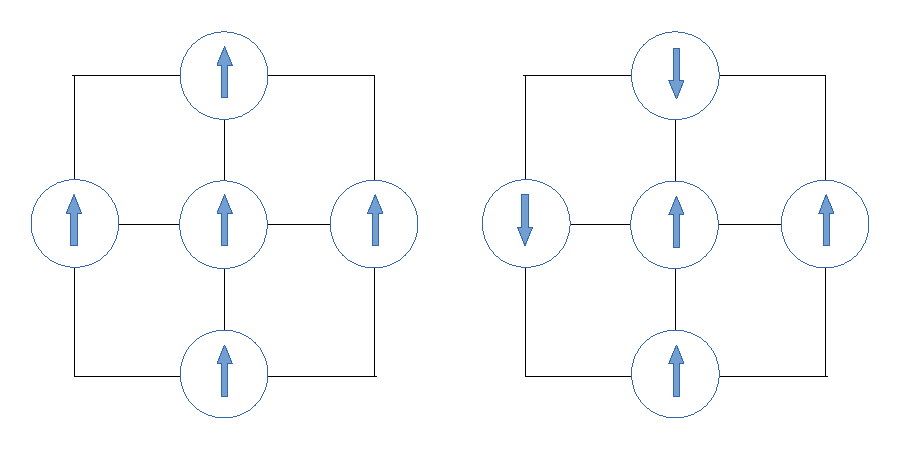
\includegraphics[width=3in]{17.Metropolis/ising1.pdf}
\caption{Examples of coupling energy.  \textit{Left}: Each f the four pairs has energy $-J$ and thus the total energy is $-4J$.  \textit{Right}:  Two pairs have energy $-J$ each and the other two pairs have $+J$ each.  Therefore, the total energy is zero.}
\label{fig:ising_model1}
\end{figure}

\bigskip
\begin{myalgobox}
\Algorithm{Monte Calro Simulation of Ising Model}\label{algo:ising}

\medskip
\begin{minipage}{5.5in}
\small
\begin{enumerate}
\item Define a 2-dimensional lattice of $L$ by $L$.  Then, $K=L^2$.  Denote the spin at the lattice point $(i,j)$ as $\sigma_{i,j}$.
\item Set an initial configuration. Any configuration is OK. For example, set $+1$ or $-1$ for each $\sigma_{i,j}$ at random.
\item Pick a candidate spin $\sigma_{i,j}$ at random. We consider flipping the spin (change the sign.)
\item Evaluate energy difference $\Delta E$ due to the flipping.
\begin{equation}
\Delta E = 2 s_{i,j} [s_{i-1,j}+s_{i+1,j}+s_{i,j-1}+s_{i,j+1}]
\end{equation}
\item If $\Delta E \le 0$, then the transition is accepted. Let $\sigma_{i,j}=-\sigma_{i,j}$. step 9.
\item If $\Delta E > 0$, generate a uniform random number $r$  between 0 and 1.
\item If $\me^{-\beta \Delta E} > r$, then the transition is accepted.  Let $\sigma_{i,j}=-\sigma_{i,j}$. step 9.
\item Otherwise, the transition is rejected.  Discard the candidate state and start over from Step 3.
\item Evaluate energy and magnetization.  Record them so that statistical average can be taken at a later time.
\item Go to Step 3 and repeat the procedure until sufficient sampling is done.
\end{enumerate}
\end{minipage}
\end{myalgobox}


Program \ref{prog:ising} simulates the  magnetization of two-dimensional Ising system isng this algorithm. The results for $40\times 40$ are shown in Figs. \ref{fig:ising_transition} --\ref{fig:ising_M_sample}.  The system size is still too small to get a good agreements with theory but the important features of the critical phenomena are realized well.


\begin{figure}
	\centering
	\begin{subfigure}{0.32\textwidth}
		\centering
		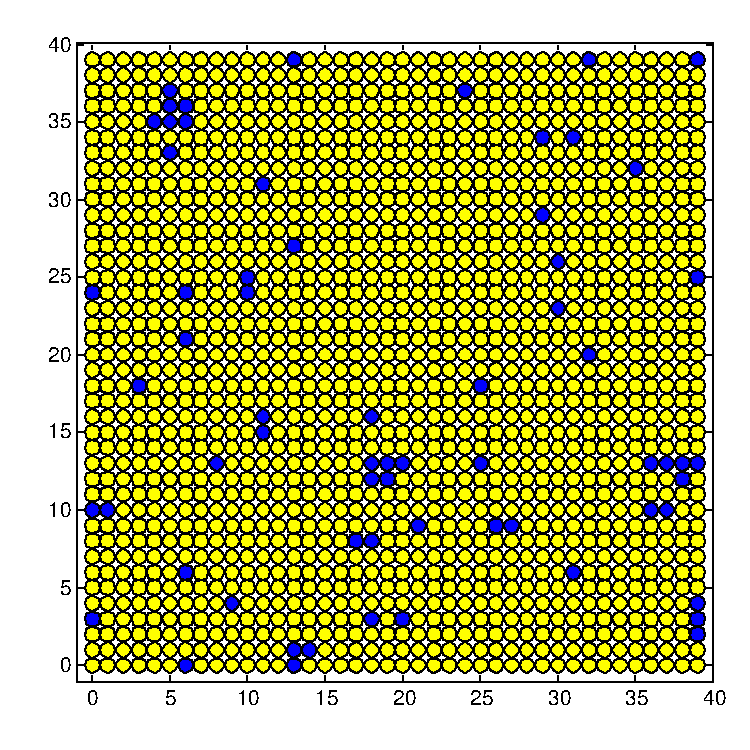
\includegraphics[width=2in]{17.Metropolis/ising_S_T=200.pdf}
		\caption{T=2.0}
	\end{subfigure}
	\begin{subfigure}{0.32\textwidth}
		\centering
		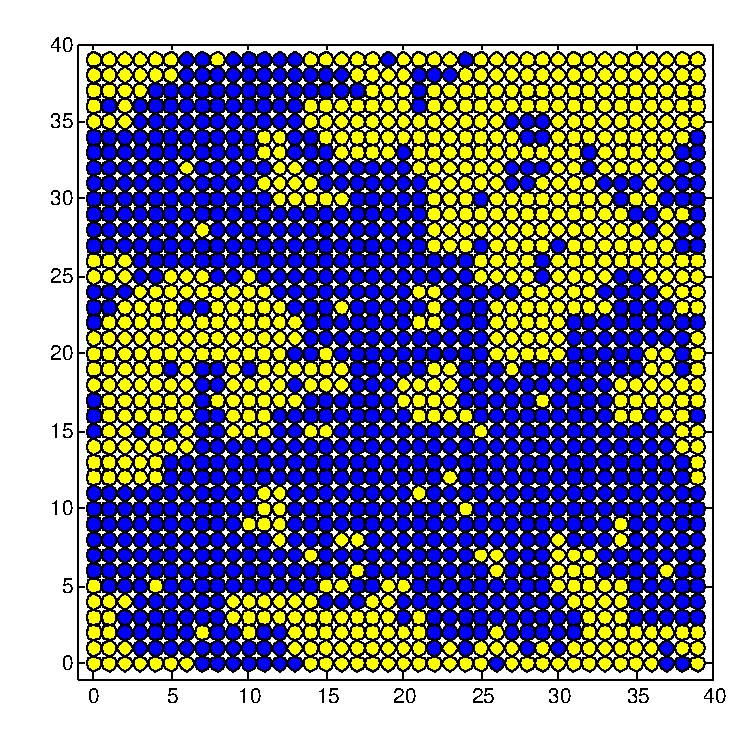
\includegraphics[width=2in]{17.Metropolis/ising_S_T=232.pdf}
		\caption{T=2.32}
	\end{subfigure}
	\begin{subfigure}{0.32\textwidth}
		\centering
		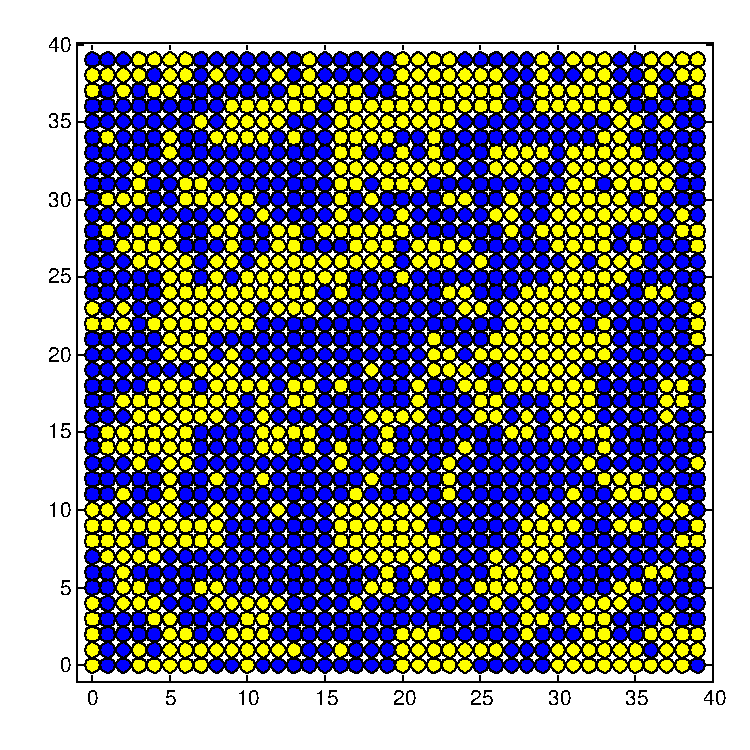
\includegraphics[width=2in]{17.Metropolis/ising_S_T=300.pdf}
		\caption{T=3.0}
	\end{subfigure}
	\caption{Snapshot of the microscopic states.  Blue sites indicate spin-up and yellow spin-down.  When temperature is well below the critical temperature (a), one color dominates. This sample happens to be dominated by yeallow but states dominated by blue also happens with the equal probability.  Well above the critical temperature (c), blue and yellow are scatted evenly.  Although a large clusters are sill seen, they should disappear as temperature goes up further.  Near the critical temperature (b),  blue and yellow are equally likely but each color forms a large cluster. along with many smaller clusters. }\label{fig:ising_S_sample}
\end{figure}

\begin{figure}
	\centering
	\begin{subfigure}{0.32\textwidth}
		\centering
		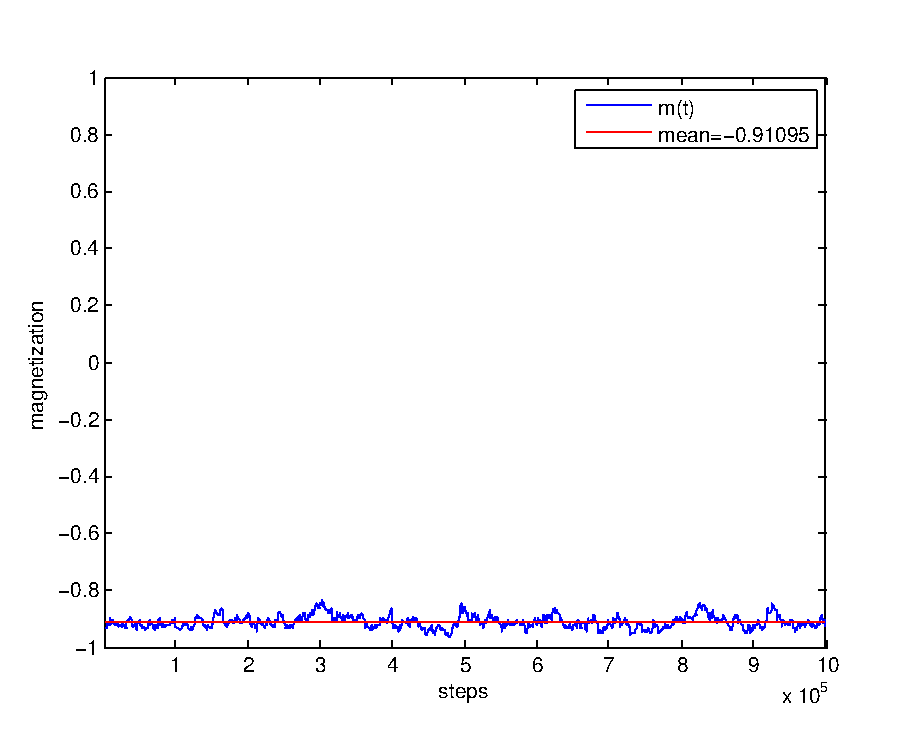
\includegraphics[width=2in]{17.Metropolis/ising_M_T=200.pdf}
		\caption{T=2.0}
	\end{subfigure}
	\begin{subfigure}{0.32\textwidth}
		\centering
		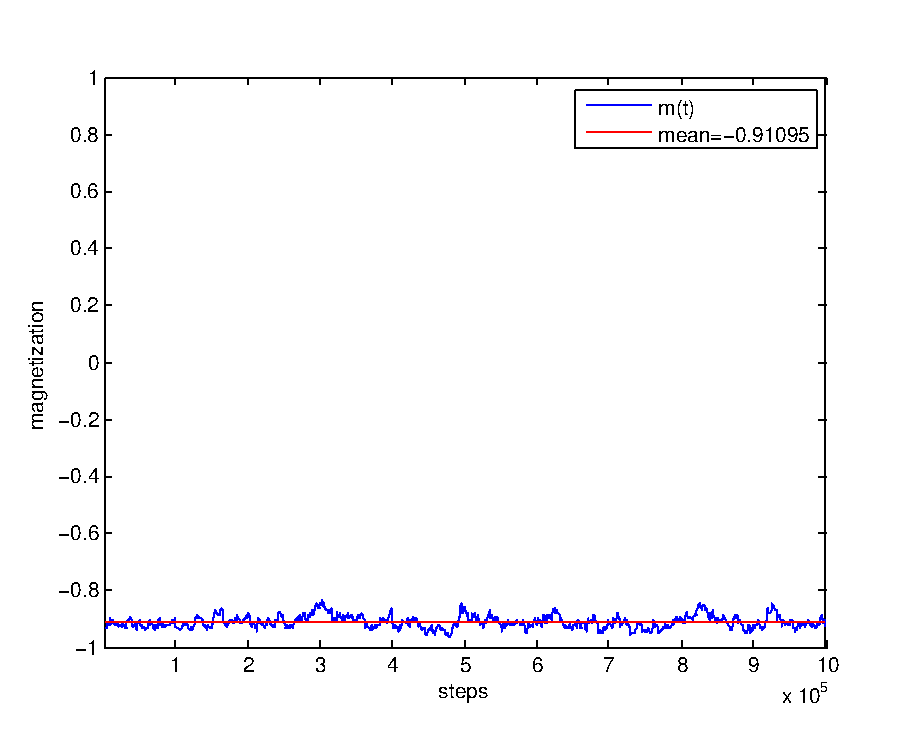
\includegraphics[width=2in]{17.Metropolis/ising_M_T=200.pdf}
		\caption{T=2.32}
	\end{subfigure}
	\begin{subfigure}{0.32\textwidth}
		\centering
		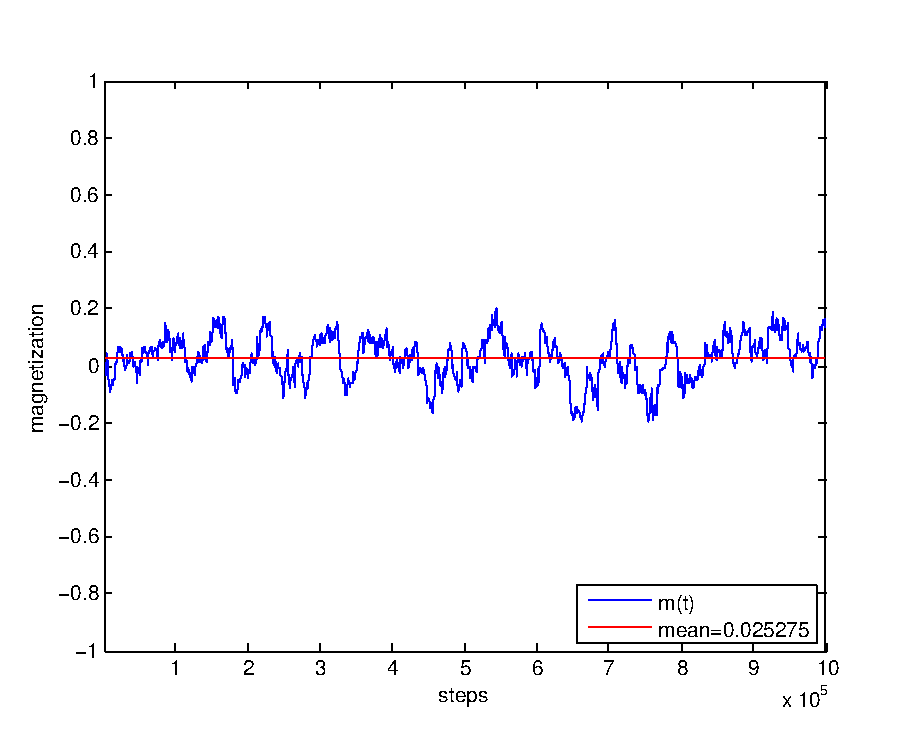
\includegraphics[width=2in]{17.Metropolis/ising_M_T=300.pdf}
		\caption{T=3.0}
	\end{subfigure}
\caption{Sampling of magnetization.  The horizontal axis indicates the individual sample.  When temperature is well below the critical temperature (a), all sampled state have similar large negative magnetization.  The flusctuation is rather small.  Well above the critical temperature (c), all sampled state have small magnetization close to zero.  The fluctuation is bigger than that of (a) due to higher temperature.  Near the critical temperature (b), each sample has quite different value of the magnetization.  The fluctuation of (b) is even larger than that of the higher temperature state (c). }\label{fig:ising_M_sample}
\end{figure}


\begin{figure}
\centering
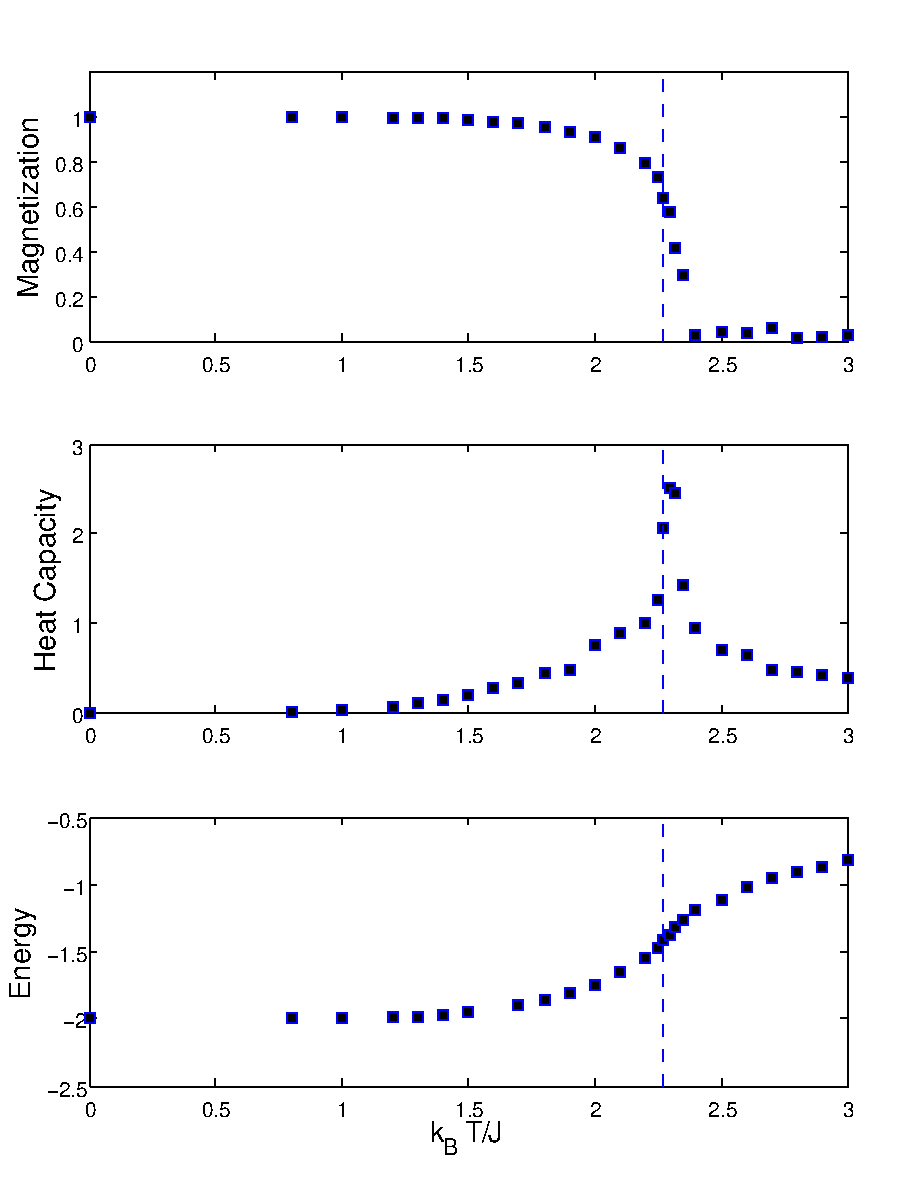
\includegraphics[width=3in]{17.Metropolis/ising_stat.pdf}
\caption{Monte Carlo Simulation of Ising model. The dashed line indicates the theoretical prediction of the critical temperature.
The top panel shows the spontaneous magnetization below a critical temperature around $T=2.4$.  The heat capacity has a sharp peak at the critical temperature as shown in the middle panel. On the other hand, the energy plotted in the bottom panel does not show any dramatic change across the transition points.}
\label{fig:ising_transition}
\end{figure}

\subsection{Percolation}

\begin{figure}
	\centering
	\begin{subfigure}{0.45\textwidth}
		\centering
		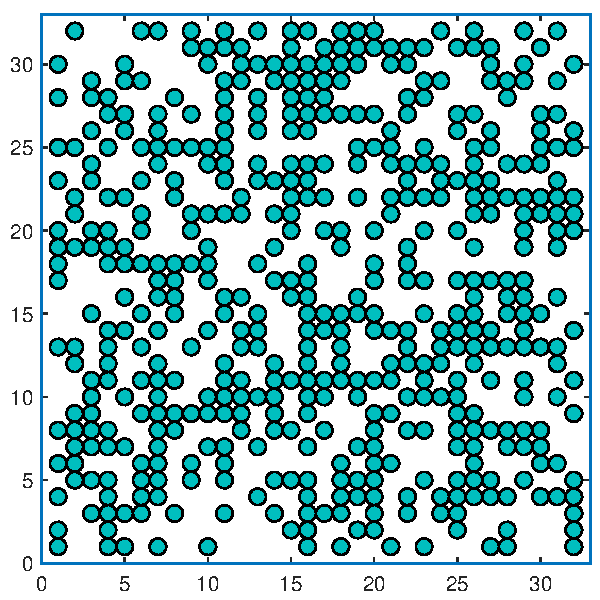
\includegraphics[width=2.5in]{17.Metropolis/perc32a.pdf}
		\caption{No percolation ($p=0.50$)}
		\label{fig:perc32a}
	\end{subfigure}
	\begin{subfigure}{0.45\textwidth}
		\centering
		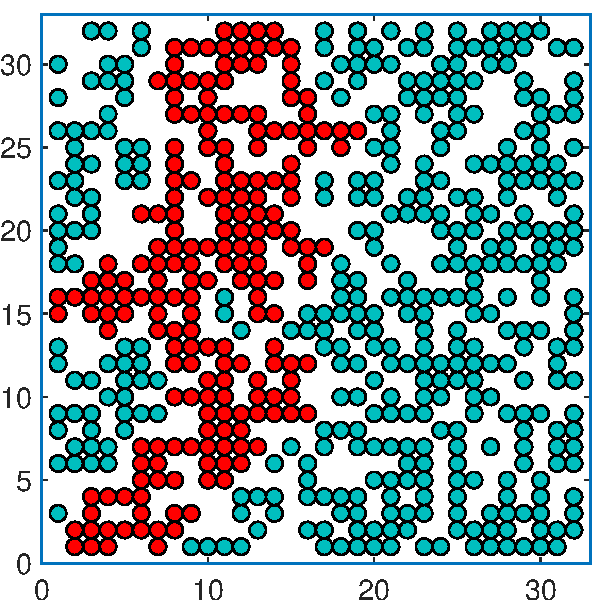
\includegraphics[width=2.5in]{17.Metropolis/perc32b.pdf}
		\caption{Vertically Percolated ($p=0.58$)}
		\label{fig:perc32b}
	\end{subfigure}
	\caption{Realization of clusters on the $32\times 32$ lattice.  No percolation is observed for $p=0.50$.  Increasing the probability to $p=0.58$, a large cluster (red) shows percolation in the horizontal direction.}
	\label{fig:perc32}
\end{figure}

The microscopic states of the two-dimensional Ising model shown in Fig. \ref{fig:ising_S_sample} show interesting geometric structures, i.e., the distribution of cluster sizes.   One interesting question is if the two opposite ends of the system is connected by a single cluster.  In other words, can we travel from one edge to the opposite edge by stepping only on one color?   For the Ising system, when temperature is sufficiently low, one color is dominated and two opposing edges are connected by a single cluster.  On the other hand, when temperature is high enough, both colors are distributed evenly and the cluster size becomes smaller. Above a certain temperature, no single cluster touches the both ends.  This phenomena is known as site percolation.\cite{percolation}  The percolation problem was originally investigated for percolation of fluids through rock.  However, it has been used for the investigation of many different systems including porous media, granular materials, the Internet, epidemics, biological evolution, to name a few.  

Now, we investigate the two-dimensional percolation by computer simulation. First, we set a rule to construct a state. Consider a $N$ by $N$ square lattice. We will place particles on the lattice at random.  The probability that a particle is found at each lattice site is $p$.   When $p=1$, then every site is occupied by a particle.If $p=0$, then there is no particle on any site.  Form $1>p>0$, some sites are occupied and other are not.  Many different configurations are possible for a given $p$.  Therefore, this system is stochastic.  To create a single configuration, generate a standard uniform random number $1>r>0$ for each lattice site.  If $p>r$, then the site is occupied.  Figure \ref{fig:perc32} shows a realization for a 32x32 lattice with $p=0.5$ and $p=0.58$.

If two adjacent sites are both occupied, then the two particles make a bond. A cluster consists of all particles connected together. 
For example,  red particles in Fig. \ref{fig:perc32b} forms a single large cluster.  There are many clusters of different sizes. The large cluster in Fig. \ref{fig:perc32b} connects the left and right edges. Therefore, this particular configuration is percolated horizontally. On theohter hand, the top and bottom edges are not connected by any cluster.  Hence, there is no vertical percolation.  In Fig. \ref{fig:perc32a}, there seems no cluster large enough to establish percolation. But it is not see that.  Actually, identifying clusters is not a trivial task for computers.  An efficient method was developed by Hoshen and Kopelman\cite{hoshen1976}.  Even fast algorithm has been developed more recently by Newman and Ziff\cite{newman2001}.  The following algorithm is based on Hoshen and Kopelman method.

We inspect each site from the bottom left corner along the column.  In Fig. \ref{fig:cluster_label}, the blue particles are already inspected and a cluster label is assigned to each cluster.  In this particular example, four clusters have been identified up to the red particle.  Now we if it is a part of a previously known cluster or a new cluster.  We don't have to worry about the grey particles at this point.  We just inspect if the red particle is in contact with any known cluster.  To do so, we need to check if two neighbor sites, one in the immediate left and the other down below.  There are five different possibilities. If neither site is occupied (Fig. \ref{fig:cluster_new}), the red particle is not in contact with any previous cluster.  It is a new cluster and we assign a new label to it.  It must be mentioned here that the assigned label is just temporary label since as the new cluster grows, it may coalesce to another cluster.  If the red particle in in contact with one known cluster (Figs. \ref{fig:cluster_left}, \ref{fig:cluster_down} and 
\ref{fig:cluster_merge1}), then assign the label of the cluster to the red particle.  


The last possibility is that the red particle is simultaneously in contact with two particles with different labels. (Fig. \ref{fig:cluster_merge2}) This is the most difficult case.  Now the clusters labeled by $n$ and $m$ coalesce to one cluster. We could simply assign a smaller label, say $m$, to the red particle.  A problem is that we need to replace all $n$ with $m$.   That is a time consuming task since we have to find all particles with label $n$.  There is a cleaver way to avoid the reassignment.  We just record the relation that the label $n$ is equivalent to the label $m$.  Such a mapping can be recorded in a one-dimensional array.  For example, if the array name is \texttt{remap}, then \texttt{remap(3)=2} indicates that the label 3 is the same as 2. If more than two labels are assigned to a single clusters, the map is chained like
\[
6 \quad \rightarrow \quad \texttt{remap(6)=4} \quad \rightarrow \quad  \texttt{remap(4)=2} \quad \rightarrow \quad \texttt{remap(2)=2}
\]
where apparent labels 6, 4, and 2 are all belong to the same cluster.  The chain of mapping ends when \texttt{remap(n)=n} is reached. We use the smallest label, 2 in this example, as the true label of the cluster.  Whenever we need the label of the particle at ($i$,$j$),  we first find the apparent label stored in a two-dimensional array
\texttt{label(i,j)}.  Then, we look for the true label by following the chain of mpping   In the case Fig. \ref{fig:cluster_merge2}, $n$ and $m$ are the apparent label.  Suppose that $m'$ and $n'$ are the true labels obtained by found through the chain of mapping.    If $n'>m'$, then assign $m'$ to the red particle.  Since the red particle and the cluster $n'$ must be mapped to the same label,  we set $\texttt{remap}(n')=m'$.  Now the label $n'$ is mapped to the same label as the red particle and thus they are in the same cluster. After this, the chain is one step longer.



\begin{figure}
	\centering
	\begin{subfigure}{0.45\textwidth}
		\centering
		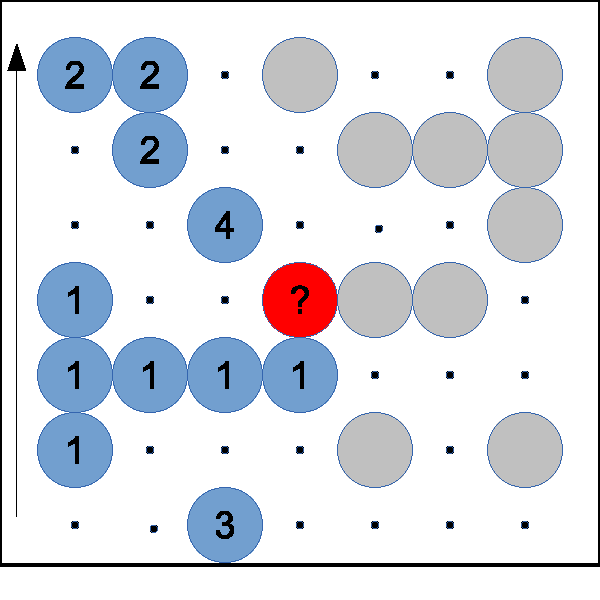
\includegraphics[width=2.0in]{17.Metropolis/cluster_labeling.pdf}
		\caption{Cluster Labeling Order}
		\label{fig:cluster_label}
	\end{subfigure}
\\
	\begin{subfigure}{0.15\textwidth}
		\centering
		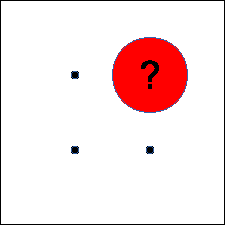
\includegraphics[width=0.7in]{17.Metropolis/cluster_new.pdf}
		\caption{ }
		\label{fig:cluster_new}
	\end{subfigure}
	\begin{subfigure}{0.15\textwidth}
		\centering
		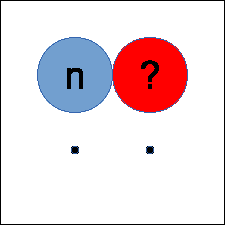
\includegraphics[width=0.7in]{17.Metropolis/cluster_left.pdf}
		\caption{ }
		\label{fig:cluster_left}
	\end{subfigure}
	\begin{subfigure}{0.15\textwidth}
		\centering
		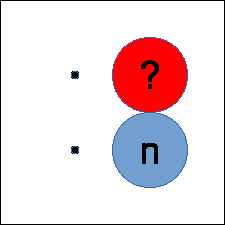
\includegraphics[width=0.7in]{17.Metropolis/cluster_down.pdf}
		\caption{}
		\label{fig:cluster_down}
	\end{subfigure}
	\begin{subfigure}{0.15\textwidth}
		\centering
		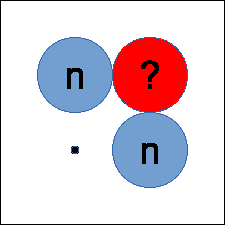
\includegraphics[width=0.7in]{17.Metropolis/cluster_merge1.pdf}
		\caption{}
		\label{fig:cluster_merge1}
	\end{subfigure}
	\begin{subfigure}{0.15\textwidth}
		\centering
		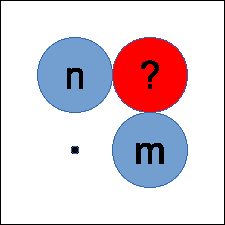
\includegraphics[width=0.7in]{17.Metropolis/cluster_merge2.pdf}
		\caption{}
		\label{fig:cluster_merge2}
	\end{subfigure}
\caption{Hoshen-Kopelman cluster labeling scheme. (a) Inspect each site from the bottom left corner along each column.  Supposed that all sites upto the red one is already inspected and a label is assigned to each cluster.  In this example, there are four clusters labeled 1 through 4.  Now we inspect if the red site is a part of the previously known cluster.  There are four five possibilities shown in (b) -- (f).}
\label{fig:cluster_labeling}
\end{figure}

\bigskip
\begin{myalgobox}
\Algorithm{Cluster Labeling}\label{algo:clusters}

\medskip
\begin{minipage}{5.5in}
\small
\begin{enumerate}
\item Prepare $N$ by $N$ array \texttt{label} for apparent labels and fill it with $0$.
\item Prepare a on-dimensional array \texttt{remap} of size $N^2$. This is used to store mapping from an apparent label to a true label.
\item Set a counter \texttt{new=0}.
\item Start with \texttt{i=1} and \texttt{j=1}, repeat the following procedure along column until \texttt{i=j=N}.
\item Check if the sites \texttt{(i-1,j)} and \texttt{(i,j-1)} is occupied.
\item If \texttt{label(i-1,j)=0} and \texttt{label(i,j-1)=0}, create a new cluster by \texttt{new=new+1}; \texttt{label(i,j)=new}; \texttt{remap(new)=new}.  Go to next site.
\item If \texttt{label(i-1,j)>0} and \texttt{label(i,j-1)=0}, join to the existing cluster by \texttt{label(i,j)=label(i-1,j)}.  Go to next site.
\item If \texttt{label(i-1,j)=0} and \texttt{label(i,j-1)>0}, join to the existing cluster by \texttt{label(i,j)=label(i,j-1)}.  Go to next site.
\item \texttt{label(i-1,j)=label(i,j-1)>0}, joint to the existing cluster by \texttt{label(i,j)=label(i-1,j)}.  Go to next site.
\item Otherwise, find the true labels \texttt{m'} and \texttt{n'} by following the chain of map.  Find the smaller/larger  of the  two true labels.  \texttt{nmin=min(m',n')} and \texttt{nmax=(m',n')}. Coalesce the two clusters into one by \texttt{label(i,j)=nmin} and \texttt{remap(nmax)=nmin}.  Go to next site.
\end{enumerate}
\end{minipage}
\end{myalgobox}


\vfill

\newpage
\noindent
\section*{MATLAB Source Codes}
\addcontentsline{toc}{section}{\protect\numberline{}MATLAB Source Codes}

\noindent
\program
\label{prog:maxwell_metropolis}
\footnotesize
\begin{verbatim}
%**************************************************************************
%*     Exercise 17.1                                                      *
%*     filename: ch17pr01.m                                               *
%*     program listing number: 17.1                                       *
%*                                                                        *
%*     This program finds the velocity distribution of one-dimensional    *
%*     ideal gas using Metropolis algorithm.                              *
%*                                                                        *
%*     Programed by Ryoichi Kawai for Computational Physics Course.       *
%*     Last modification:  03/11/2017.                                    *
%**************************************************************************
clear all
close all

N0=10000;  % number of thermalization steps
N=200000;  % number of samples
kT=1.0;    % Temperature times Boltzmann constant
m=1.0;     % mass
dv=0.1;    % maximum jump in velocity

v0=sqrt(kT/m); % thermal speed
v(1)=2.0*v0*(rand(1)-0.5); % initial velocity (radom between -0.5 and _0.5)

for i=1:N+N0-1
    found = false;
    while not(found)
        u = v(i) + dv*(2*rand(1)-1);   % candidate
        dE = m/2*(u^2-v(i)^2);         % energy change
        if exp(-dE/kT)>rand(1)            % accept or reject
            v(i+1)=u;
            found = true;
        end
    end
end

K=41;
h=histogram(v(N0+1:N+N0),K,'Normalization','pdf');
hold on
w=linspace(h.BinLimits(1),h.BinLimits(2),101);
y=1/sqrt(2*pi*kT/m) * exp(-m*w.^2/(2*kT));
% theoretical distribution (Maxwell)
p=plot(w,y);
set(p,'color','red','linewidth',2);
legend(p,'Maxwell');
hold on
legend('show')
axis([-4 4 0 0.5])
hold off
\end{verbatim}
\normalsize

\noindent
\program
\label{prog:ising}
\footnotesize
\begin{verbatim}
%**************************************************************************
%*     Exercise 17.2                                                      *
%*     filename: ch17pr02.m                                               *
%*     program listing number: 17.2                                       *
%*                                                                        *
%*     This program simulates two-dimensional Ising model using           *
%*     the Metropolis algorithm.                                          *
%*                                                                        *
%*     Programed by Ryoichi Kawai for Computational Physics Course.       *
%*     Last modification:  03/17/2017.                                    *
%**************************************************************************
clear all
close all

rng('shuffle')

% control parameters
L=32;         % number of spins in one direction
LL=L*L;       % total number of spins
N0=20000;     % thermalization steps
N=1000000;    % number of Metropolis steps.
NS=N/1000;    % number of samples.

% temperature
T=2.0;       
beta = 1/T;

% Define arrays
kmax=int32(N/NS);
m=zeros([kmax,1]);
sigma2=zeros([kmax,1]);
E=zeros([kmax,1]);

% animation switch
movie=false;

if T>2.0
    s = int32(1-2*randi([0,1],[L,L]));   % Random (for high temperature)
else
    s = int32(ones([L,L]));              % Uniform (for low temperature)
end

% animation initial configuration
if movie
    figure
    axis([0 L+1 0 L+1])
    axis equal;
    hold on
    for i=1:L
        for j=1:L
            if s(i,j)>0
                color='blue';
            else
                color='yellow';
            end
            rectangle('Position',[i,j,1,1],'Curvature',[1 1],'FaceColor',color);
        end
    end
    drawnow;
end

% Begin Metropolis simulation 
k=0;
for n=1:N+N0
    % pick a site at random 
    i=randi([1,L]);
    j=randi([1,L]);

    % Evaluation of energy change
    i1=i+1; if i1>L;  i1=1; end;
    i2=i-1; if i2<1;  i2=L; end;
    j1=j+1; if j1>L;  j1=1; end;
    j2=j-1; if j2<1;  j2=L; end;
    s4 = s(i1,j)+s(i2,j)+s(i,j1)+s(i,j2);
    dE = 2.0*double(s4*s(i,j));

% Metropolis algorithm
    if exp(-beta*dE)> rand(1)
        s(i,j)=-s(i,j);  
        if movie
            if s(i,j)>0
                color='blue';
            else
                color='yellow';
            end
            rectangle('Position',[i,j,1,1],'Curvature',[1 1],'FaceColor',color);
            drawnow;
        end
    end
    
% measurement
    if n>N0 && mod(n,NS)==0
        k=k+1;
        m(k) = sum(s(:))/LL;                % mean magnetization
        sigma2(k) = sum(s(:).^2)/LL-m(k)^2; % variance
        % total energy
        h=0;
        for j=1:L-1
            for i=1:L-1
                 h=h+s(i,j)*(s(i+1,j)+s(i,j+1));
            end
        end
        for i=1:L
            h=h+s(i,L)*s(i,1)+s(L,i)*s(1,i);
        end
        E(k)=-h;
    end

end

% draw the final configuration
if not(movie)
    figure
    axis([0 L+1 0 L+1])
    axis equal;
    hold on
    for i=1:L
        for j=1:L
            if s(i,j)>0
                color='blue';
            else
                color='yellow';
            end
            rectangle('Position',[i,j,1,1],'Curvature',[1 1],'FaceColor',color)
        end
    end

    hold off
   drawnow;
end

% magnetization
subplot(1,2,1)
plot([1:k]*NS,m(1:k))
hold on
mu=sum(m(1:k))/k;
p=plot([NS, k*NS],[mu, mu]);
set(p,'color','red')
axis([0 N -1.1 1.1])
mx=num2str(mu,5);
legend('m(t)',['mean=' mx])
legend('location','southeast')
xlabel('steps')
ylabel('magnetization')
hold off

% energy
subplot(1,2,2)
Eavg=sum(E)/k;
C=(sum(E.^2)/k-Eavg^2)/T^2/LL;
p=plot([1:k]*NS,E(1:k)/LL);
hold on
p=plot([NS, k*NS],[Eavg/LL, Eavg/LL]);
set(p,'color','red')
axis([0 N -4 0])
mx=num2str(Eavg/LL,5);
legend('E(t)',['mean=' mx])
xlabel('steps')
ylabel('Energy/spin')
hold off

% statistics
fprintf('<m>=%.5f\n',mu)
fprintf('<E>=%.5f\n',Eavg/LL)
fprintf('<C>=%.5f\n',C)
\end{verbatim}
\normalsize

\noindent
\program
\label{prog:percolation}
\footnotesize
\begin{verbatim}
%**************************************************************************
%*     Exercise 17.3                                                      *
%*     filename: ch17pr03.m                                               *
%*     program listing number: 17.3                                       *
%*                                                                        *
%*     This program simulates two-dimensional percolation.                *
%*     Hoshen and Kopelman algorithm is used for cluster labeling.        *
%*                                                                        *
%*     Programed by Ryoichi Kawai for Computational Physics Course.       *
%*     Last modification:  03/17/2017.                                    *
%**************************************************************************
close all

N=32;
% p=0.59 is close to the transition point
p=0.4;

% Graphics setting
plot([0,N+1,N+1,0,0],[0,0,N+1,N+1,0]);
axis equal
axis([0 N+1 0 N+1])
hold on

% place atoms at random
r=rand(N,N);
lattice = r < p;

% draw clusters
for i=1:N
    for j=1:N
        if lattice(i,j)
            rectangle('Position',[i,j,1,1],'Curvature',[1 1],'FaceColor','b');
            drawnow
        end
    end
end
hold on


% Labeling: 1st pass (Making initial labels and map)

label=zeros(N,N);  % allocate array
remap=zeros(N*N);

new=0;
for j=1:N
    for i=1:N
        
        i1 = i-1;
        j1 = j-1;
        
        if lattice(i,j)>0
            if i1 > 0
                left=label(i1,j); % neighbor (left).
            else
                left=0;  % outside the box.
            end
            if j1 > 0
                down=label(i,j1); % neighbor (down).
            else
                down=0;  % outside the box.
            end
            
            if down==0 && left==0  % if both are unocupied
                new=new+1;         % create a new cluster.
                label(i,j) = new;
                remap(new)=new;
                
            elseif down*left>0  % both are occupied.
                
                if down==left        % if they are the same cluster.
                    label(i,j)=left; % join to the cluster.
                    
                else   % connecting two different clusters.
                    found = false;
                    while not(found)
                        if remap(left)==left
                            found = true;
                        else
                            left=remap(left);
                        end
                    end
                    found = false;
                    while not(found)
                        if remap(down)==down
                            found = true;
                        else
                            down=remap(down);
                        end
                    end
                    
                    if left==down  % they are again the same
                        label(i,j)=left;
                    else
                        nmax=max(left,down);
                        nmin=min(left,down);
                        label(i,j)=nmin;   % coalesce two clusters
                        remap(nmax)=nmin;  % add to the chain
                    end
                end
                
            elseif down>0 % only down neighbor is occupied
                label(i,j) = down;  % join to the neighbor
                
            else  % only the left neighbor is occupied
                label(i,j) = left;  % join to the neighbor
            end
        end
        
    end
end
% Labeling: 2nd pass (Collapse the label in the same cluster)

nmax = max(label(:));
for i=nmax:-1:1
    label(label==i)=remap(i);
end

% Labeling: 3rd pass (Make the label continuous)
%           This procedure is not essential.

j=0;
for i=1:nmax
    if remap(i)==i
        j=j+1;
        label(label==i) = j;
    end
end

% Identify the percolation
nmax = max(label(:));
size = zeros(nmax,1);
maxsize=0;
largest=1;
fprintf('Cluster   Size  Percolation\n')
for i=1:nmax
    percx = any(label(1,:)==i)*any(label(N,:)==i) >0;
    percy = any(label(:,1)==i)*any(label(:,N)==i) >0;
    size(i)=  sum(label(:)==i);
    if size(i) > maxsize
        largest = i;
        maxsize = size(i);
    end
    if percx || percy
        perc='YES';
    else
        perc=' NO';
    end
    fprintf('%5d:  %6d,    %s\n', i, size(i), perc)
end

fprintf('%d    %d\n', largest, size(largest))

for i=1:N
    for j=1:N
        if label(i,j) == largest
            rectangle('Position',[i,j,1,1],'Curvature',[1 1],'FaceColor','r');
            drawnow
        end
    end
end
figure

h=histogram(size,20);
\end{verbatim}
\normalsize

\ruleend

\bigskip
\noindent
\section*{Python Source Codes}
\addcontentsline{toc}{section}{\protect\numberline{}Python Source Codes}
\setcounter{program}{0}

\bigskip
\noindent
\program
\footnotesize
\begin{verbatim}
#!/usr/bin/env python3
# -*- coding: utf-8 -*-
"""
%**************************************************************************
%*     Exercise 17.1                                                      *
%*     filename: ch17pr01.m                                               *
%*     program listing number: 17.1                                       *
%*                                                                        *
%*     This program finds the velocity ditribution of one-dimensional     *
%*     ideal gas using Metropolis algorithm.                              *
%*                                                                        *
%*     Programed by Ryoichi Kawai for Computational Physics Course.       *
%*     Last modification:  03/11/2017.                                    *
%**************************************************************************
"""

import numpy as np
import matplotlib.pyplot as plt

N0=10000 # number of thermalization steps
N=200000; # number of samples
kT=3.0 # Temperature times Boltzmann constant
m=5.0 # mass of particle

v=np.zeros(N+N0)
dv=0.1    # maximum jump in velocity
v0=np.sqrt(kT/m)   # thermal speed
# initial velocity (uniform random beteen -v0 and +v0)
v[0]=2.*v0*(np.random.rand(1)-0.5)  

for i in range(0,N+N0-1):
    found = False
    while not(found):
        u = v[i] + dv*(2.0*np.random.rand(1)-1.0)   # candidate
        dE = m/2.0*(u**2-v[i]**2)           # energy change
        if np.exp(-dE/kT)>np.random.rand(1):    # Metropolis condition
            v[i+1]=u                         # accept change ()
            found = True

# theoretical distribution (Maxwell)
K=41
plt.close()
plt.figure(figsize=(6,5))
n, bins, patches = plt.hist(v[N0:N0+N],K,normed=1,label='Monte Carlo')
w=np.linspace(bins[0],bins[-1],101)
y=1.0/np.sqrt(2.*np.pi*kT/m) * np.exp(-m*w**2/(2.*kT))
plt.plot(w,y,'-r',label='Maxwell')
plt.legend(loc=1)
plt.xlabel('v')
plt.ylabel('p(v)')
plt.show()
\end{verbatim}
\normalsize

\ruleend

\bigskip
\noindent
\program
\footnotesize
\begin{verbatim}
#!/usr/bin/env python3
# -*- coding: utf-8 -*-
"""
%**************************************************************************
%*     Exercise 17.2                                                      *
%*     filename: ch17pr02.py                                              *
%*     program listing number: 17.2                                       *
%*                                                                        *
%*     This program simulates two-dimensional Ising model using           *
%*     the Metropolis algorithm.                                          *
%*                                                                        *
%*     Programed by Ryoichi Kawai for Computational Physics Course.       *
%*     Last modification:  03/17/2017.                                    *
%**************************************************************************
"""
import numpy as np
import matplotlib.pyplot as plt

# ease all previous figures
plt.close('all')

# control parameters
L=32          # number of spins in one direction
LL=L*L        # total number of spins
N0=20000      # thermalization steps
N=100000      # number of Metropolis steps.
NS=N/1000     # number of samples.

# Define arrays
kmax=np.int(N/NS)
m=np.zeros(kmax)
sigma2=np.zeros(kmax)
E=np.zeros(kmax)

# Show animation if True
movie=False

# temperature
T=2.0        
beta = 1.0/T

# Initial configuration
if T>2.0:
    # Random (for high temperature)
    s=np.random.choice([1,-1],[L,L])
else:
    # Uniform (for low temperature)
    s=np.ones((L,L),dtype=np.int)

#  Show initial configuration
if movie:
    plt.figure(figsize=(6,6))
    plt.axis('equal')
    plt.axes(xlim=(-1, L), ylim=(-1, L))
    for j in range(0,L):
        for i in range(0,L):
            if s[i,j]==1:
                color='b'
            else:
                color='y'
            circle=plt.Circle((i,j),0.5,fc=color)
            plt.gca().add_patch(circle)
    plt.pause(0.0001)

# Begin Metropolis simulation    
k=0
for n in range(0,N+N0):
    # pick a site at random 
    i=np.random.randint(0,L)
    j=np.random.randint(0,L)

    # Evaluation of energy change
    i1=np.mod(i+1,L)
    i2=np.mod(i-1,L)
    j1=np.mod(j+1,L)
    j2=np.mod(j-1,L)
    ss = s[i1,j]+s[i2,j]+s[i,j1]+s[i,j2]
    dE = 2*ss*s[i,j]

# Flip spin based on Metropolis algorithm
    if np.exp(-beta*dE)> np.random.rand(1):
        s[i,j]=-s[i,j]

        # Show new configuration
        if movie:
            if s[i,j]==1:
                color='b'
            else:
                color='y'
            circle=plt.Circle((i,j),0.5,fc=color)
            plt.gca().add_patch(circle)
            plt.pause(0.0001)
            
    # Evaluate statistical quantities
    if n>N0 and np.mod(n,NS)==0:
        
        # mean and variance
        m[k] = np.real(s.sum())/LL
        sigma2[k] = (s**2).sum()/LL-m[k]**2 

        # total nergy
        h=0
        for j in range(0,L-1):
            for i in range(0,L-1):
                 h=h+s[i,j]*(s[i+1,j]+s[i,j+1])
        for i in range(0,L):
            h=h+s[i,L-1]*s[i,0]+s[L-1,i]*s[0,i]
        E[k]=-h

        k+=1

# plot magnetization
plt.figure(figsize=(12,5))
plt.subplot(1,2,1)
t=np.linspace(0,k-1,k)*NS
plt.plot(t,m[0:k],'-b',label='m(t)')

mu=sum(m[1:k])/k
plt.plot([0, N],[mu, mu],'--r',label='mean')
plt.xlim([0,N])
plt.ylim([-1.1,1.1])
plt.legend(loc=4)
plt.xlabel('steps')
plt.ylabel('magnetization')

# plot energy
plt.subplot(1,2,2)
Eavg=sum(E[0:k])/k
C=(sum(E[0:k]**2)/k-Eavg**2)/T**2/LL
plt.plot(t,E[0:k]/LL,label='energy');
plt.plot([0,N],[Eavg/LL, Eavg/LL],'--r',label='mean')
plt.xlim([0,N])
plt.ylim([-4,0])
plt.xlabel('steps')
plt.ylabel('Energy/spin')
plt.show()

# Show the final configulation
if not(movie):
    plt.figure(figsize=(6,6))
    plt.axis('equal')
    plt.axes(xlim=(-1, L), ylim=(-1, L))
    for j in range(0,L):
        for i in range(0,L):
            if s[i,j]==1:
                color='b'
            else:
                color='y'
            circle=plt.Circle((i,j),0.5,fc=color)
            plt.gca().add_patch(circle)
    plt.show()
    
# statistics
print('<m>={0:8.5f}'.format(mu))
print('<E>={0:8.5f}'.format(Eavg/LL))
print('<C>={0:8.5f}'.format(C))
\end{verbatim}
\normalsize

\ruleend
\bigskip
\noindent
\program
\footnotesize
\begin{verbatim}
#!/usr/bin/env python3
# -*- coding: utf-8 -*-
"""
%**************************************************************************
%*     Exercise 17.3                                                      *
%*     filename: ch17pr03.m                                               *
%*     program listing number: 17.3                                       *
%*                                                                        *
%*     This program simulates two-dimensional percolation.                *
%*     Hoshen and Kopelman algorithm is used for cluster labeling.        *
%*                                                                        *
%*     Programed by Ryoichi Kawai for Computational Physics Course.       *
%*     Last modification:  03/17/2017.                                    *
%**************************************************************************
"""
import numpy as np
import matplotlib.pyplot as plt

# ease all previous figures
plt.close('all')

N=32
# p=0.59 is close to the transition point
p=0.59

# Graphics setting
plt.figure(figsize=(6,6))
plt.axis('equal')
plt.axes(xlim=(-1, N), ylim=(-1, N))

# place atoms at random
r=np.random.rand(N,N)
lattice = r < p

# draw clusters
for i in range(0,N):
    for j in range(0,N):
        if lattice[i,j]:
            circle=plt.Circle((i,j),0.5,fc='b')
            plt.gca().add_patch(circle)
            plt.pause(0.0001)

# Labeling: 1st pass (Making initial labels and map)
label=np.zeros([N,N],dtype=np.int)  # allocate array
remap=np.zeros(N*N,dtype=np.int)

new=0
for j in range(0,N):
    for i in range(0,N):
        
        i1 = i-1
        j1 = j-1
        
        if lattice[i,j]>0:
            if i1 < 0:
                left=0            # outside the box
            else:
                left=label[i1,j]  # left neighbor

            if j1 < 0:
                down=0            # outside the box.
            else:
                down=label[i,j1]  # down neighbor
            
            if down==0 and left==0:  # if both are unocupied
                new=new+1            # create a new cluster.
                label[i,j]=new
                remap[new]=new
                
            elif down*left>0:       # both are occupied.
                
                if down==left:      # if they belong to the same cluster.
                    label[i,j]=left # join to the cluster.
                    
                else:               # connecting two different clusters.
                    found = False
                    while not(found):
                        if remap[left]==left:
                            found = True
                        else:
                            left=remap[left]

                    found = False
                    while not(found):
                        if remap[down]==down:
                            found = True
                        else:
                            down=remap[down]
                    
                    if left==down:     # they again belong to the same
                        label[i,j]=left
                    else:
                        nmax=np.max([left,down])
                        nmin=np.min([left,down])
                        label[i,j]=nmin    # coalesce two clusters
                        remap[nmax]=nmin   # add to the chain
                
            elif down>0:            # only down neighbor is occupied
                label[i,j] = down   # join to the neighbor
                
            else:                   # only the left neighbor is occupied
                label[i,j] = left   # join to the neighbor

# Labeling: 2nd pass (Collapse the label in the same cluster)

nmax = np.max(label)
for i in range(nmax,0,-1):
    label[label==i]=remap[i]

# Labeling: 3rd pass (Make the label continuous)
#          This procedure is not essential.
j=0
for i in range(1,nmax+1):
    if remap[i]==i:
        j=j+1
        label[label==i] = j

# Find cluster size and find percolation
nmax = np.max(label)
size = np.zeros(nmax+1,dtype=np.int)
maxsize=0
largest=1
print('Cluster   Size  Percolation')
for i in range(1,nmax+1):
    percx = any(label[0,:]==i)*any(label[N-1,:]==i) >0
    percy = any(label[:,0]==i)*any(label[:,N-1]==i) >0
    size[i]= (label==i).sum()
    if size[i] > maxsize:
        largest = i
        maxsize = size[i]

    if percx or percy:
        perc='YES'
    else:
        perc=' NO'

    print('{0:5d}:  {1:5d},    {2:s}'.format(i, size[i], perc))

# Show the largest cluster
for i in range(0,N):
    for j in range(0,N):
        if label[i,j] == largest:
            circle=plt.Circle((i,j),0.5,fc='r')
            plt.gca().add_patch(circle)
            plt.pause(0.0001)

# Plot size distribution
plt.figure(figsize=(6,5))
plt.hist(size,maxsize)
plt.show()
\end{verbatim}
\normalsize

\ruleend

\vfill

\newpage
%\chapbibliography
\bibliographystyle{unsrt}
\bibliography{compphys}